\documentclass{article}
\usepackage{tabularx}
\usepackage{longtable}
\usepackage{array}
\usepackage{float}
\usepackage{listings}
\usepackage{amsmath}
\usepackage{amssymb}
\usepackage{mathtools}
\usepackage{amsfonts}
\usepackage{graphicx}
\usepackage[table]{xcolor}
\setlength{\arrayrulewidth}{0.5mm}
\graphicspath{ {./images/} }
\usepackage[margin=20mm]{geometry}
\renewcommand{\labelenumii}{\theenumii}
\renewcommand{\theenumii}{\theenumi.\arabic{enumii}.}
\renewcommand{\arraystretch}{1.5}
\newcommand{\f}[2]{f_{#1}(#2)}
\newcommand{\code}[1]{\texttt{#1}}
\DeclarePairedDelimiter{\ceil}{\lceil}{\rceil}
\DeclarePairedDelimiter{\set}{\left\{}{\right\}}
\DeclarePairedDelimiter{\parens}{\lparen}{\rparen}
\title{HW3 Report}
\date{}
\begin{document}
\maketitle
\section*{Section 1}
\subsection*{Q1:}
    \begin{figure}[H]
        \centering
        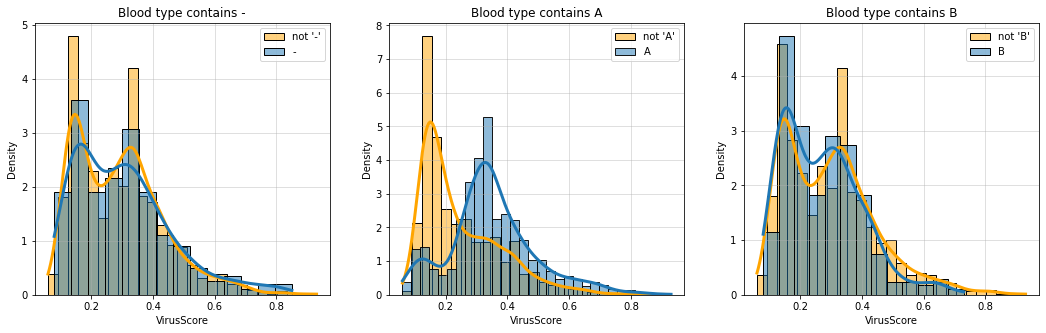
\includegraphics[scale=0.5]{images/q1.png}
        \caption{KDE plots of \code{VirusScore} conditioned different conditions of \code{blood\_type}}
        \label{fig:q1}
    \end{figure}
\subsection*{Q2:}
    \paragraph*{}
    In figure \ref{fig:q1} in the plot of A versus not A, we observe that the groups of patients with and and without "A" in their blood types are mostly seperable along a boundary that is approximately the \code{VirusScore} of $0.225$. 
    \paragraph*{}
    Therefore, the condition of contains/does not contain A would be most informative for learning \code{VirusScore}.
    As it turns out, we decided already in hw1 to create this feature.
\subsection*{Q3:}
    \begin{figure}[H]
        \centering
        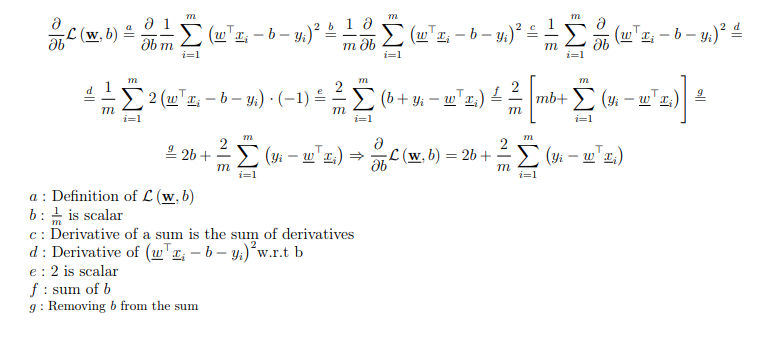
\includegraphics[scale=0.7]{images/q3.png}
    \end{figure}
\subsection*{Q4:}
    \begin{figure}[H]
        \centering
        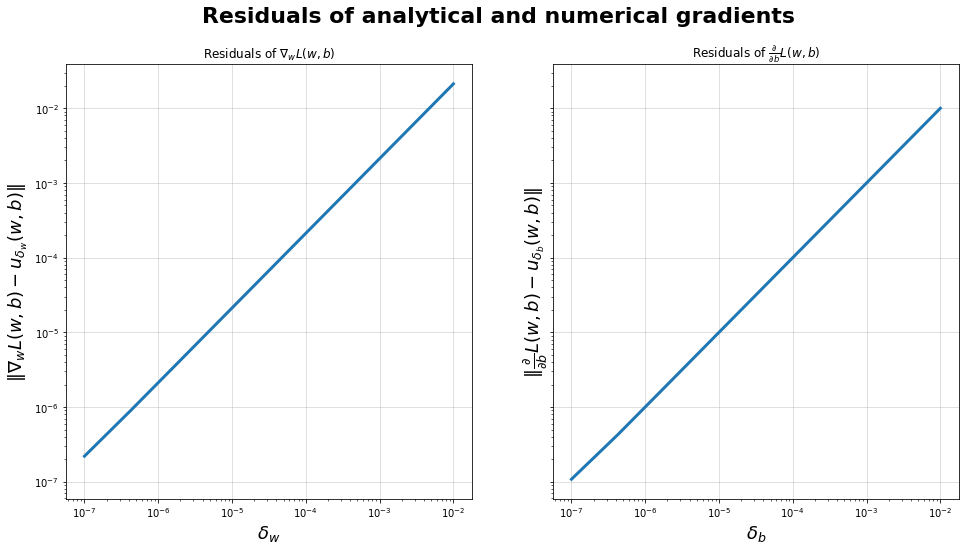
\includegraphics[scale=0.48]{q4.png}
        \caption{Plot of Residuals of analytical and numerical gradients}
        \label{fig:q4}
    \end{figure}
    \paragraph*{}
    As we can see in figure \ref{fig:q4}, the difference between the analytic and numerical gradients increases in a  monotonic fashion as the value of $\delta$ increases. This is logical, as $\delta$ is the differential size used in the definition of the numerical gradient, and therefore a smaller $\delta$  equates to a more precise estimation of the analytic gradient by the numerical gradient.
\subsection*{Q5:}
    \begin{figure}[H]
        \centering
        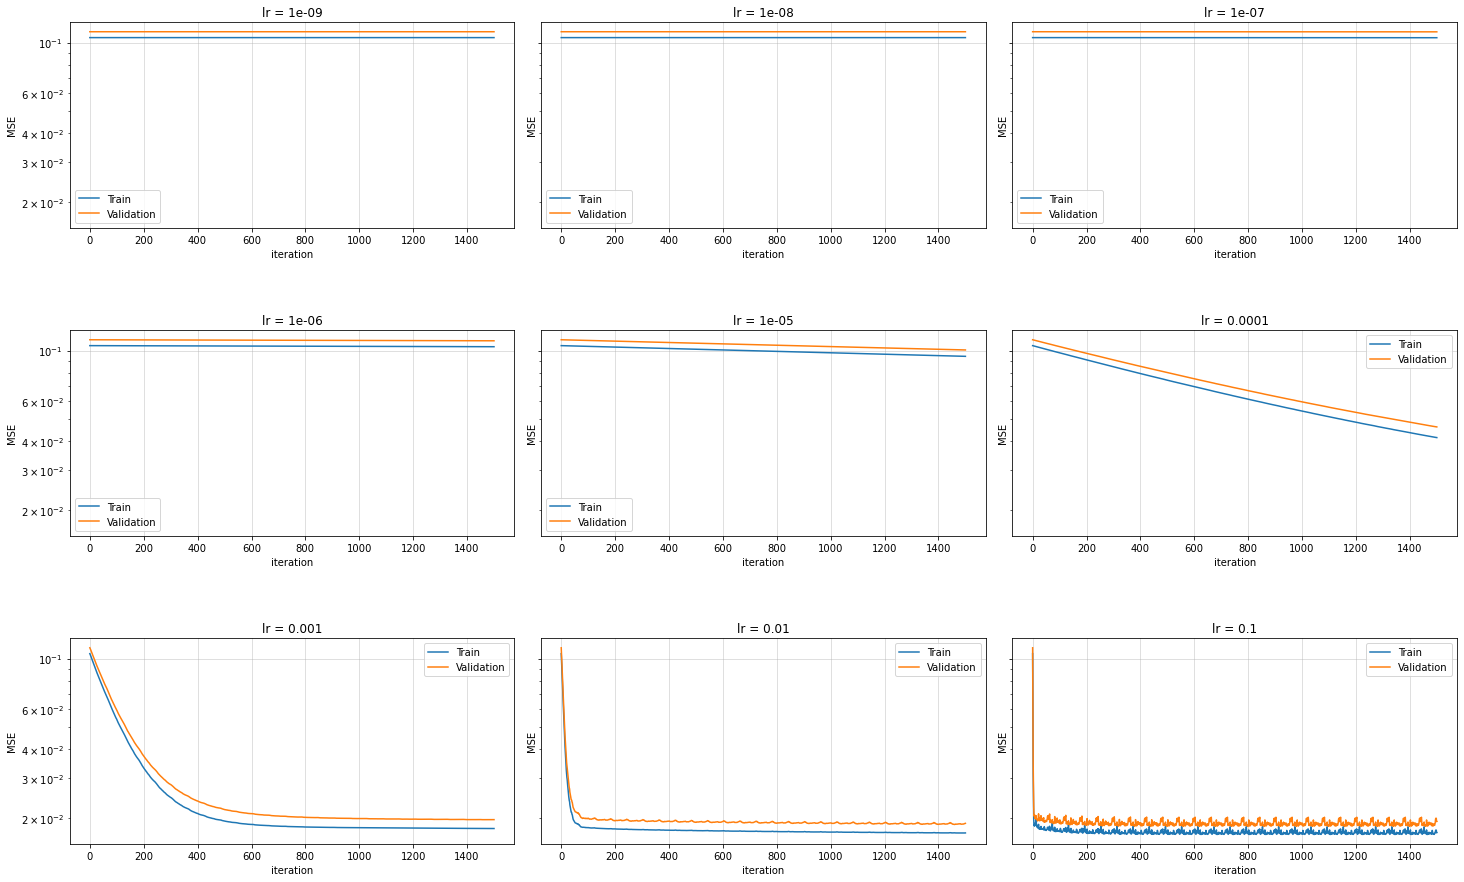
\includegraphics[scale=0.35]{q5.png}
        \caption{Graphs of Training and Validation Losses as Functions of Iteration Number for Different  Learning Rates}
        \label{fig:q5}
    \end{figure}
    \paragraph*{}
    We can see in figure \ref{fig:q5} that for smaller lr, for those that converge, the convergence is at a higher loss for both the training and validation. This matches the theory, since if the lr is too small, the SGD algorithm is likely to converge to a sub-optimal solution. In addition we observe that for the lr equal to $0.1$ the graphs do not converge for both training and validation losses and for lr equal to $0.01$ the validation loss does not converge, which fits the theory that says that learning rates that are too high are likely to cause the SGD algorithm to take steps that are too large and thus repeatedly skip-over the optimal solution. This points to $0.001$ as being the optimal lr, as both the validation and training losses converge to values that are substantially lower than the next smaller lr.
\subsection*{Q6:}
    \begin{figure}[H]
        \centering
        \begin{tabular}{|c|c|c|c|}
            \hline
            \rowcolor{gray!60}
            Model & Section & Train MSE & Valid MSE\\ \hline
            \rowcolor{gray!20}
            ~&~ & \multicolumn{2}{c|}{Cross Validated}\\ \hline
            Dummy & 3 & $0.0204$ & $0.0205$\\ \hline
        \end{tabular}
        \caption{Training and Validation MSE Errors for Dummy Regressor}
    \end{figure}
\section*{Section 4}
\subsection*{Q7:}
    \begin{figure}[H]
        \centering
        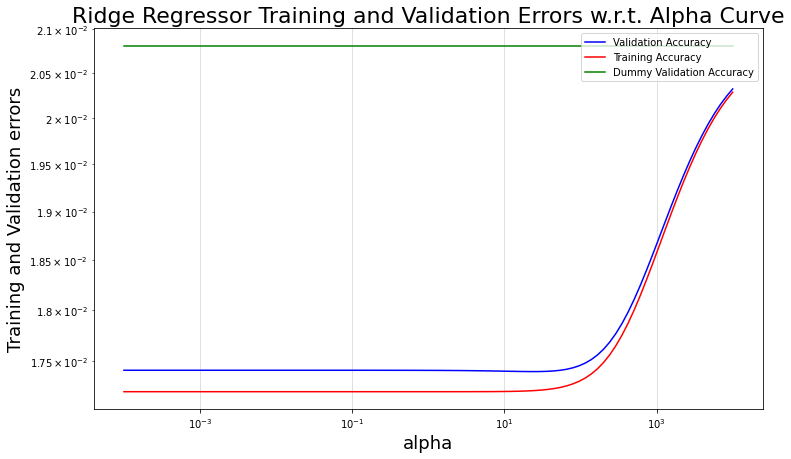
\includegraphics[scale=0.5]{q7.png}
        \caption{Graph of Training and Validation Errors of Ridge Regressor as a Function of \code{alpha}}
        \label{fig:q7}
    \end{figure}
    Optimal alpha for validation: 25.950242113997373\\
    Validation error for optimal alpha: 0.017402908351734445

\subsection*{Q8:}
    \begin{figure}[H]
        \centering
        \begin{tabular}{|c|c|c|c|}
            \hline
            \rowcolor{gray!60}
            Model & Section & Train MSE & Valid MSE\\ \hline
            \rowcolor{gray!20}
            ~&~ & \multicolumn{2}{c|}{Cross Validated}\\ \hline
            Dummy & 3 & $0.0204$ & $0.0205$\\ \hline
            Ridge linear & 4 & $0.0172$ & $0.0174$\\ \hline
        \end{tabular}
        \caption{Training and Validation MSE Errors for Dummy and Ridge Regressors}
    \end{figure}
\subsection*{Q9:}
    \begin{figure}[H]
        \centering
        \begin{tabular}{|c|c|}
            \hline
            \rowcolor{gray!60}
            Feature & Coefficient \\ \hline
            \code{blood\_A\_AB} & $0.0970$ \\ \hline
            \code{num\_of\_siblings} & $0.0298$ \\ \hline
            \code{household\_income} & $-0.0275$ \\ \hline
            \code{PCR\_02} & $-0.0141$ \\ \hline
            \code{PCR\_01} & $-0.0113$ \\ \hline
        \end{tabular}
        \caption{Five Features From Ridge Regressor With Largest Coefficients in Terms of Absolute Value, From Largest to Smallest}
    \end{figure}
\subsection*{Q10:}
    \begin{figure}[H]
        \centering
        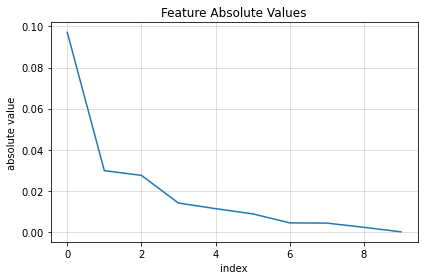
\includegraphics[scale=0.7]{q10.png}
        \caption{Graph of Absolute Values of Learned Coefficients of Ridge Regressor}
        \label{fig:q10}
    \end{figure}
\section*{Section 5}
\subsection*{Q11:}
    \begin{figure}[H]
        \centering
        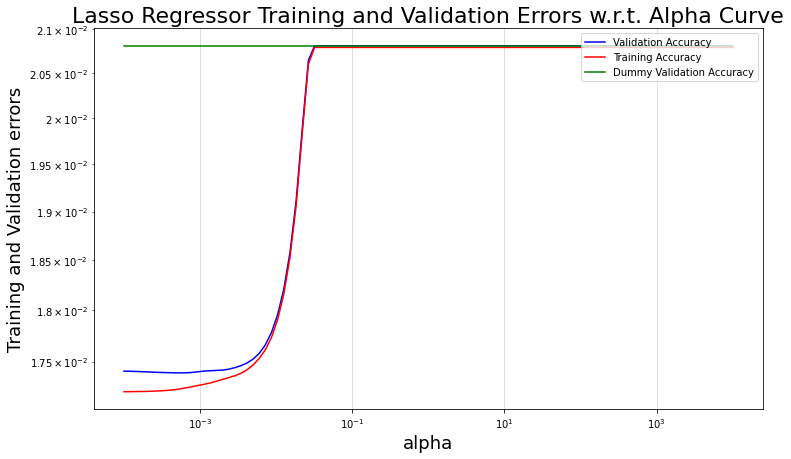
\includegraphics[scale=0.5]{q11.png}
        \caption{Graph of Training and Validation Errors of Lasso Regressor as a Function of \code{alpha}}
        \label{fig:q11}
    \end{figure}
    Optimal alpha for validation: 0.0005336699231206312\\
    Validation error for optimal alpha: 0.01739141826673015

\subsection*{Q12:}
    \paragraph*{}
    Yes, the graph for tunning the $\lambda$ of the lasso regressor as can be seen in figure \ref{fig:q11} is different from the graph obtained for the ridge regressor in figure \ref{fig:q7} in a number of aspects.
    \paragraph*{}
    Firstly, the steepness of the upwards curve is much more abrupt and significant in the case of the lasso regressor than it is for the ridge. This can be explained by the way in which lasso differs than ridge: Whereas a ridge regressor utilizes $\ell^2$ regularization, lasso is implemented with $\ell^1$. This means that as $\lambda$ (\code{alpha}) is increased, the weight coefficients for the two regressors decrease in different manners. In the case of ridge, the coefficients experience weight decay, meaning they gradually tend to zero, whereas lasso tends to perform variable selection, meaning that the coefficients are more abruptly forced to zero one-by-one. This is reflected in the graphs, as the abruptness seen in figure \ref{fig:q11} could be explained by a certain significant coefficient abruptly forced to zero, whereas in the ridge graph of figure \ref{fig:q7}, coefficients are more gradually lowered and therefore the curve is more gradual.
    \paragraph*{}
    Furthermore, the upwards trend in the graph of lasso begins at a much lower \code{alpha} approximately equal to $0.025$ than it does for ridge (approximately \code{alpha} equal to $70$). This can be again explained by the behavior of $\ell^1$ as opposed to $\ell^2$: The decision of the lasso regressor to decrease a significant coefficient would be more abrupt and harsher than in the case of ridge, and therefore its effect on the accuracy would be seen almost immediately, and hence the earlier upwards trend in the lasso graph.
    \paragraph*{}
    Lastly, the optimal \code{alpha} for minimal validation error in thew case of lasso, equal to $0.0005$, is much smaller than that of ridge ($25.95$).


\subsection*{Q13:}
    \begin{figure}[H]
        \centering
        \begin{tabular}{|c|c|c|c|}
            \hline
            \rowcolor{gray!60}
            Model & Section & Train MSE & Valid MSE\\ \hline
            \rowcolor{gray!20}
            ~&~ & \multicolumn{2}{c|}{Cross Validated}\\ \hline
            Dummy & 3 & $0.0204$ & $0.0205$\\ \hline
            Ridge linear & 4 & $0.0172$ & $0.0174$\\ \hline
            Lasso linear & 5 & $0.0172$ & $0.0173$\\ \hline
        \end{tabular}
        \caption{Training and Validation MSE Errors for Dummy, Ridge, and Lasso Regressors}
    \end{figure}
\subsection*{Q14:}
    \begin{figure}[H]
        \centering
        \begin{tabular}{|c|c|}
            \hline
            \rowcolor{gray!60}
            Feature & Coefficient \\ \hline
            \code{blood\_A\_AB} & $0.0993$ \\ \hline
            \code{num\_of\_siblings} & $0.0297$ \\ \hline
            \code{household\_income} & $-0.0223$ \\ \hline
            \code{PCR\_02} & $-0.0064$ \\ \hline
            \code{PCR\_10} & $0.0038$ \\ \hline
        \end{tabular}
        \caption{Five Features From Lasso Regressor With Largest Coefficients in Terms of Absolute Value, From Largest to Smallest}
    \end{figure}
\subsection*{Q15:}
    \begin{figure}[H]
        \centering
        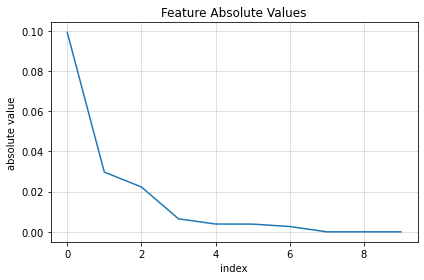
\includegraphics[scale=0.7]{q15.png}
        \caption{Graph of Absolute Values of Learned Coefficients of Lasso Regressor}
        \label{fig:q15}
    \end{figure}
    \paragraph*{}

\section*{Section 6}
\subsection*{Q16:}
    \paragraph*{}
    When using a polynomial feature mapping, we can expect the training error to decrease and the validation error to increase. This is because the polynomial mapping will give more flexibility to the regression model to more closely try to fit the training data during training in a polynomial way, thereby leading to lower training error, but also causing overfitting and therefore leading to a higher validation error.

\subsection*{Q18:}
    \begin{figure}[H]
        \centering
        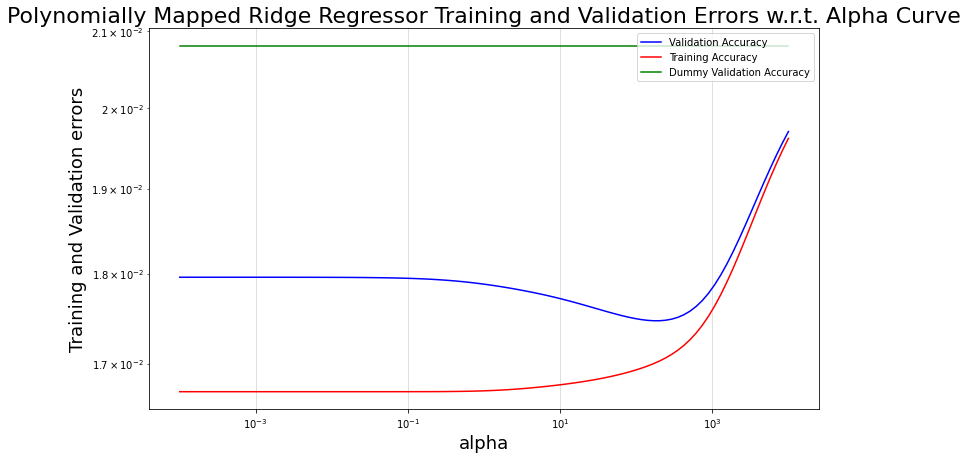
\includegraphics[scale=0.5]{q18.png}
        \caption{Graph of Training and Validation Errors of Polynomially-Mapped Ridge Regressor as a Function of \code{alpha}}
        \label{fig:q8}
    \end{figure}
    Optimal alpha for validation: 200.923300256505\\
    Validation error for optimal alpha: 0.01747015013288799

\subsection*{Q19:}
    \begin{figure}[H]
        \centering
        \begin{tabular}{|c|c|c|c|}
            \hline
            \rowcolor{gray!60}
            Model & Section & Train MSE & Valid MSE\\ \hline
            \rowcolor{gray!20}
            ~&~ & \multicolumn{2}{c|}{Cross Validated}\\ \hline
            Dummy & 3 & $0.0204$ & $0.0205$\\ \hline
            Ridge linear & 4 & $0.0172$ & $0.0174$\\ \hline
            Lasso linear & 5 & $0.0172$ & $0.0173$\\ \hline
            Ridge polynomial & 6 & $0.0166$ & $0.0174$\\ \hline
        \end{tabular}
        \caption{Training and Validation MSE Errors for Dummy, Ridge, Lasso, and Polynomial Ridge Regressors}
    \end{figure}

\section*{Section 7}
\subsection*{Q20:}
    \begin{figure}[H]
        \centering
        \begin{tabular}{|c|c|c|c|c|}
            \hline
            \rowcolor{gray!60}
            Model & Section & Train MSE & Valid MSE & Test MSE\\ \hline
            \rowcolor{gray!20}
            ~&~ & \multicolumn{2}{c|}{Cross Validated} & Retrained \\ \hline
            Dummy & 3 & $0.0204$ & $0.0205$ & $0.0182$\\ \hline
            Ridge linear & 4 & $0.0172$ & $0.0174$ & $0.0163$\\ \hline
            Lasso linear & 5 & $0.0172$ & $0.0173$ & $0.0162$\\ \hline
            Ridge polynomial & 6 & $0.0166$ & $0.0174$ & $0.0164$\\ \hline
        \end{tabular}
        \caption{Training, Validation, and Test MSE Errors for Dummy, Ridge, Lasso, and Polynomial Ridge Regressors}
        \label{fig:q20}
    \end{figure}
\end{document}